\question{Задача о перпендикуляре.}

\begin{multicols}{2}
  \begin{figure}[H]
  \centering
  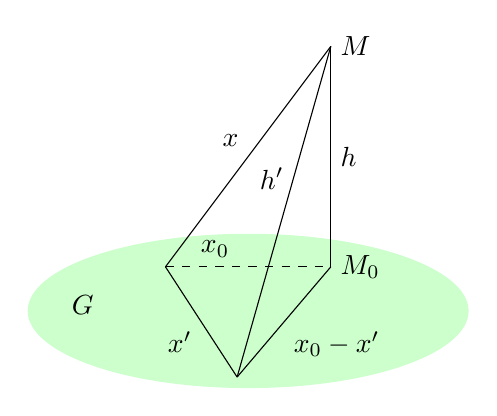
\begin{tikzpicture}[scale = 0.7]
    
    \fill[green!20] (1.5, -0.8) ellipse (4cm and 1.4cm);

    \draw (0, 0) -- (3, 4) node[midway, above left] {\(x\)};
    \draw[dashed] (0, 0) -- (3, 0) node[pos = 0.3, above] {\(x_{0}\)};
    \draw (3, 0) -- (3, 4) node[midway, right] {\(h\)};
    \draw (0, 0) -- (1.3, -2) node[midway, below left] {\(x'\)};
    \draw (1.3, -2) -- (3, 0) node[midway, below right] {\(x_{0} - x'\)};
    \draw (1.3, -2) -- (3, 4) node[pos = 0.6, left] {\(h'\)};

    \draw node[right] at (3, 4) {\(M\)};
    \draw node[right] at (3, 0) {\(M_{0}\)};
    \draw node at (-1.5, -0.7) {\(G\)};

  \end{tikzpicture}
\end{figure}
  \columnbreak

  \underline{Постановка задачи}: необходимо найти перпендикуляр
  \(h \perp G \colon x_{0} + h = x \; (x_{0} \in G, x \in E^{n})\), т.е. нужно
  найти точку \(M_{0}\)~--- проекцию \(M\) на \(G\).

  В таком случае \(x_{0}\) называется \textit{ортогональной} проекцией \(x\) на
  \(G\).

  \begin{theorem}
    В описанных выше условиях \(h\) задает кратчайшее расстояние от \(x\) до
    \(G\):

    \begin{align*}
      \forall x' \in G \mid x' \neq x_{0} \colon
        \under{\abs{x - x'}}{h'} > \under{\abs{x - x_{0}}}{h}
    \end{align*}
  \end{theorem}
\end{multicols}

\begin{proof}
  \begin{align*}
    \begin{rcases}
      x', x_{0} \in G \implies x_{0} - x' \in G \\
      h \perp G
    \end{rcases}
    \implies h \perp (x_{0} - x') \\
    \norm{h'}^2
    = \norm{x - x'}^2
    = \norm{x - x_{0} + x_{0} - x'}
    \eqby{\ref{pythagoras}}
    \under{\norm{x - x_{0}}^2}{\norm{h}^2} + \norm{x_{0} - x'}
    \\
    \norm{h'}^2 = \norm{h}^2 + \norm{x_{0} - x'}
    \\
    x' \neq x_{0}
    \implies \norm{x_{0} - x'} > 0
    \implies \norm{h'}^2 > \norm{h}^2
  \end{align*}
\end{proof}

\begin{remark}
  \(x_{0}\) это проекция \(x\) на \(G\), отстоящая от \(x\) на наименьшее
  расстояние.
\end{remark}

\begin{remark}
  О вычислении ортогональной проекции

  В \(G\) выделим базис \(\Basis\) и разложим \(x_{0}\) по этому базису:

  \begin{align*}\label{eq:ort-proj-calc-1}\tag{1}
    x_{0} = \lambda_{1} \basis_{1} + \dotsc + \lambda_{k} \basis_{k}
  \end{align*}

  Теперь задача состоит в поиске коэффициентов \(\lambda_{i}\).
  воспользуемся тем, что \(h\) это перпендикуляр к \(G\):

  \begin{align*}\label{eq:ort-proj-calc-2}\tag{2}
    \begin{rcases}
      h = x - x_{0} \\
      h \perp G \bydef \forall \basis_{i} \in \Basis \colon h \perp \basis_{i}
    \end{rcases}
    \implies (x - x_{0}, \basis_{i}) = 0
    \implies (x_{0}, \basis_{i}) = (x, \basis_{i})
    \hspace{20pt} (\forall \basis_{i} \in \Basis)
  \end{align*}

  Подставим \eqref{eq:ort-proj-calc-1} в \eqref{eq:ort-proj-calc-2} и
  воспользуемся свойствами скалярного произведения:

  \begin{align*}
    \forall \basis_{i} \in \Basis \colon
      \lambda_{1} (\basis_{1}, \basis_{i}) + \dotsc
        + \lambda_{n} (\basis_{n}, \basis_{i})
      = (x, e_{i})
  \end{align*}

  Для каждого \(\basis_{i} \in \Basis\) получаем свое уравнение \(\implies\)
  можно составить СЛАУ:

  \begin{align*}
    \begin{pmatrix}
      (\basis_{1}, \basis_{1}) & \dots  & (\basis_{k}, \basis_{1}) \\
      \vdots                   & \ddots & \vdots                   \\
      (\basis_{1}, \basis_{k}) & \dots  & (\basis_{k}, \basis_{k}) \\
    \end{pmatrix}
    \begin{pmatrix}
      \lambda_1 \\ 
      \vdots \\
      \lambda_k
    \end{pmatrix}
    =
    \begin{pmatrix}
      (x, \basis_{1}) \\
      \vdots \\
      (x, \basis_{k})
    \end{pmatrix}
  \end{align*}
\end{remark}

Заметим, что матрица коэффициентов полученной СЛАУ это матрица Грамма.
По т. Крамера эта СЛАУ будет иметь единственное решение, если
\(\det \Gmtx \neq 0\).
